\chapter{Methodology}
\label{chapter:methods}


\begin{introduction}
\begin{flushright}
``Without action, the best intentions in the world are nothing more than that: intentions.''
\end{flushright}

\vspace{0.5em}

This chapter details the methodological design of the study. Three portfolio optimization frameworks are introduced, DRL--PPO, LSTM--BL, and LSTM--SR, each evaluated under four feature variants that progressively incorporate sentiment signals derived from financial news and social media. The shared experimental conditions, cross-validation strategy, and feature engineering pipeline are described to ensure transparency and reproducibility. Two classical benchmark strategies are also included for reference.
\end{introduction}


Considering the objective of this work, three distinct frameworks were implemented, each comprising four variants, alongside two benchmark strategies for comparison. The use of multiple frameworks is motivated by the need to explore different paradigms for portfolio optimization, particularly given the lack of consensus in the literature regarding a dominant approach, as discussed in Section \ref{section:portfolio_optimization}. Within each framework, four variants were developed to evaluate the contribution of different feature sets and their impact on model performance, particularly the inclusion of features based on sentiment analysis.

An initial split between training and test datasets was performed, as summarized in Table~\ref{tab:train_test_split}. The training period spans from the second semester of 2015 to the first semester of 2023, while the test period covers the second semester of 2023 to the first semester of 2025. This division provides a sufficiently long historical window for model training while preserving a recent and relevant period for out-of-sample evaluation. Furthermore, using a common test period ensures that all frameworks and benchmark models are evaluated under identical market conditions, enabling a fair and consistent comparison of their performance.

\begin{table}[ht]
\centering
\caption{Training and Test Periods (Semesters)}
\label{tab:train_test_split}
\begin{tabular}{|c|c|}
\hline
\textbf{Training Period} & \textbf{Test Period} \\
\hline
S2 2015--S1 2023 (8 years) & S2 2023--S1 2025 (2 years) \\
\hline
\end{tabular}
\end{table}

\section{Portfolio Optimization Frameworks}

To ensure comparability across all frameworks, all proposed approaches were developed under a consistent set of shared conditions and constraints.

Regarding the portfolio constraints, positions are restricted to long-only, portfolios must remain fully invested at all times, with daily rebalancing, and bid-ask spreads must be applied as transaction costs. These constraints are chosen to strike a balance between reflecting realistic investment conditions faced by practitioners and maintaining methodological comparability with the reviewed literature. The long-only constraint is particularly relevant for equity portfolios, where short-selling may be restricted or undesirable. The fully invested requirement ensures that the models are evaluated on their ability to allocate capital effectively rather than on their ability to time cash holdings. Daily rebalancing allows the models to respond to changing market conditions and capture short-term signals, motivated also by the daily cadence of the available data. Bid-ask spreads prevent the models from exploiting unrealistic trading strategies that would not be viable in practice, such as excessive turnover or frequent small adjustments that would incur prohibitive transaction costs. By incorporating these constraints, the frameworks are designed to produce results that are not only theoretically sound but also practically relevant and implementable in real-world trading scenarios.

Regarding the experimental conditions, the frameworks are required to handle assets with partial histories, annual refitting to new data, hyperparameter selection, feature engineering, and a cross-validation strategy for robust evaluation and tuning. The partial histories condition arises because some assets in the investment universe have inception dates that fall within the training period, resulting in missing observations at the start of the sample. The annual refitting condition is necessary to account for non-stationarity in financial markets, as models need to adapt to evolving market dynamics rather than relying on a fixed, potentially stale, parameter set. Hyperparameter selection and feature engineering are crucial for optimizing model performance, but they must be conducted carefully to avoid overfitting to the training period. Finally, a cross-validation strategy is essential for robust evaluation and tuning, as it allows for a more reliable assessment of the model's performance and helps in selecting the best hyperparameters for each approach.

For all the frameworks, the cross-validation strategy implemented is an expanding-window walk-forward validation, as commonly used in the financial machine learning literature. This approach involves training the model on an initial period of data, then validating it on a subsequent period, and iteratively expanding the training window while moving forward through time \cite{0df79, lopezdeprado2018afml_ch1}. Specifically, three folds were created within the training period, each with its own training, early stopping, and validation periods. The early stopping period is used to monitor the performance of the model during training and to prevent overfitting by stopping the training process when the performance on the early stopping set starts to degrade. The validation period is used to evaluate the performance of the model after training and to select the best model based on its performance on this set. This cross-validation strategy allows for a more reliable assessment of the model's performance and helps in selecting the best hyperparameters for each approach. The specific periods for each fold are detailed in Table~\ref{tab:train_val_periods}.

This yearly refit and early stopping strategy is also applied during test set evaluation. The model is refitted annually, once before the July 2023--June 2024 period and once before the July 2024--June 2025 period. Each refit uses all data available up to that point, with the most recent year reserved as an early stopping validation set. This prevents overfitting to the latest observations while still allowing the model to adapt to evolving market conditions, though at the cost of excluding that final year from the training signal.

\begin{table}[ht]
\centering
\caption{Training, Early Stopping, and Validation Periods per Fold (Semesters)}
\label{tab:train_val_periods}
\begin{tabular}{|c|c|c|c|}
\hline
\textbf{Fold} & \textbf{Training Period} & \textbf{Early Stop Period} & \textbf{Validation Period} \\
\hline
1 & S2 2015--S1 2019 (4 years) & S2 2019--S1 2020 (1 year) & S2 2020--S1 2021 (1 year) \\
2 & S2 2015--S1 2020 (5 years) & S2 2020--S1 2021 (1 year) & S2 2021--S1 2022 (1 year) \\
3 & S2 2015--S1 2021 (6 years) & S2 2021--S1 2022 (1 year) & S2 2022--S1 2023 (1 year) \\
\hline
\end{tabular}
\end{table}

Having established the common constraints and experimental conditions, the following sections present the three proposed frameworks: Deep Reinforcement Learning with Proximal Policy Optimization (DRL--PPO), Long Short-Term Memory networks used for return prediction within a Black-Litterman optimization framework (LSTM--BL), and Long Short-Term Memory networks trained to directly optimize the Sharpe ratio (LSTM--SR).

\subsection{Deep Reinforcement Learning with Proximal Policy Optimization (DRL--PPO)}
% https://claude.ai/chat/8fb0d396-1af9-4b3a-a38d-66bc4f4d4caa

This framework implements a deep reinforcement learning (DRL) approach to portfolio optimization, where an agent learns to allocate capital across a universe of assets by interacting with a trading environment. This approach is inspired by the work of Sood \emph{et al.}~\cite{0df79}, which demonstrated the potential of DRL for dynamic portfolio allocation. The core idea is to train a Proximal Policy Optimization (PPO) agent, a state-of-the-art policy gradient method, to directly optimize a reward signal that reflects the financial objective of interest, such as risk-adjusted returns.

The overall system is modular in design: the trading environment, the neural network architecture, the reward function, and the optimization procedure are each independently encapsulated but share the same code paths between the hyperparameter search stage and the final training run. This guarantees that the configuration selected during tuning is evaluated under conditions identical to those of the final model.

\paragraph{Trading Environment} The agent interacts with a custom environment that implements the Gymnasium interface, the standard abstraction for reinforcement learning environments. At each discrete time step, the agent receives a structured observation of the current market state and outputs a vector of real-valued logits, one per asset. These logits are passed through a masked softmax transformation that converts them into a valid long-only portfolio weight vector. The masking operation works by setting the logit of any asset flagged as unavailable at that step to negative infinity before the softmax is applied, which forces its output weight to exactly zero regardless of the original logit value. The remaining weights sum to one by the properties of softmax, guaranteeing a fully invested, leverage-free allocation at every step without requiring any explicit constraint on the action space. Transaction costs (bid-ask spreads) are incorporated at each rebalancing step as a function of portfolio turnover, penalizing excessive trading and encouraging the agent to learn allocation strategies that are stable over time.

\paragraph{Reward} The reward signal follows a two-phase structure designed to balance learning stability with the ultimate objective of risk-adjusted performance. During an initial warm-up period, the agent is rewarded based on net portfolio returns. This phase allows the policy to develop a basic understanding of return dynamics before a more demanding objective is imposed. After the warm-up, the reward transitions linearly to the Differential Sharpe Ratio (DSR). The DSR provides an online, incremental approximation of the Sharpe ratio gradient, eliminating the need for a fixed lookback window~\cite{dsratio, 0df79}. To prevent numerical instability from extreme returns, the reward is clipped to a symmetric range. The momentum parameter, clipping range, and warm-up duration are treated as tunable hyperparameters rather than fixed design choices.

\paragraph{States} At each time step, the agent receives a structured observation consisting of a three-dimensional tensor of shape $[\text{lookback} \times N \times F]$, representing a rolling window of $F$ features for each of the $N$ assets over a lookback window, along with the previous portfolio weights, a binary availability mask indicating which assets are tradable at that step, and an optional scalar market signal. Flattening this heterogeneous observation for a standard multilayer perceptron (MLP) would discard the per-asset structure and force the network to learn asset-specific representations implicitly, incurring a substantial parameter cost.

\paragraph{Actions} The action space is a continuous vector of dimension $N$, where each element corresponds to the portfolio weight assigned to one asset. The agent is constrained to long-only, fully invested allocations: all weights are non-negative and sum to one at every step, with no leverage or short positions permitted. Assets flagged as unavailable in the observation mask receive zero weight by construction.

\paragraph{Neural Network Architecture} To process the structured observation efficiently, the model employs a permutation-equivariant feature extractor as the network head. Each asset's feature window is passed independently through a shared MLP encoder with Tanh activation, ensuring the representation generalizes across assets and keeping the parameter count independent of $N$. The per-asset embeddings are aggregated across the asset dimension using max-pooling, which retains the strongest signals while avoiding dilution of high-performing assets. The pooled embedding is concatenated with the market signal, previous portfolio weights, and availability mask, and the resulting vector is fed to a shared MLP, which splits into actor and critic heads of the PPO network. The actor head produces a logit per asset which, after a masked softmax, yields the final portfolio weights, and the critic head produces a scalar state-value estimate used to compute generalized advantage estimates during the policy update.

% \paragraph{Policy Optimization} At each iteration of the training procedure, the agent collects a fixed number of interactions from a single environment into a rollout buffer. The use of a single environment is a deliberate choice: financial time series are strictly sequential, and parallelizing across multiple environments would require careful management of temporal overlap, introducing inconsistencies between the hyperparameter search and the final training regime. Once the buffer is full, it is divided into mini-batches, and the PPO objective is optimized for a fixed number of epochs. The loss combines three terms: the clipped surrogate policy loss, which constrains each policy update to remain within a trust region defined by the clip range parameter, the value function loss, which trains the critic to accurately predict future returns, and an entropy bonus, which penalises overly deterministic policies and encourages continued exploration throughout training. The relative weight of the entropy bonus is controlled by a coefficient that is itself subject to hyperparameter search, as its optimal value is sensitive to both the structure of the action space and the stage of training.
\paragraph{Policy Optimization} At each iteration of the training procedure, the agent collects a fixed number of interactions from a single environment into a rollout buffer. The use of a single environment is a deliberate choice: financial time series are strictly sequential, and parallelizing across multiple environments would require careful management of temporal overlap, introducing inconsistencies between the hyperparameter search and the final training regime. Once the buffer is full, it is divided into mini-batches, and the PPO objective is optimized for a fixed number of epochs. The loss, $\mathcal{L}(\theta) = \mathcal{L}^{\text{CLIP}}(\theta) - c_1\mathcal{L}^{\text{VF}}(\theta) + c_2\mathcal{H}[\pi_\theta]$, following the standard PPO formulation, combines three terms: the clipped surrogate policy loss, $\mathcal{L}^{\text{CLIP}}(\theta)$, which constrains each update via a probability ratio $r_t(\theta)$ clipped to $[1-\epsilon, 1+\epsilon]$, the value function loss, $\mathcal{L}^{\text{VF}}(\theta)$, which trains the critic to predict future returns, and an entropy bonus, $\mathcal{H}[\pi_\theta]$, which discourages premature convergence to deterministic policies. The loss coefficients are treated as hyperparameters and tuned during the search procedure, along with the clipping threshold $\epsilon$, as their optimal values are sensitive to the specific financial application, the structure of the action space, and the stage of training.

\paragraph{Hyperparameter Optimization} The full set of hyperparameters is optimized towards maximizing the mean annualized Sharpe ratio averaged across multiple random seeds and validation folds, which explicitly rewards configurations that are robust across different initializations and market regimes. The search space covers all major dimensions of the model: the core PPO algorithm parameters, namely the discount factor, the Generalized Advantage Estimation (GAE) lambda governing the bias-variance trade-off in advantage estimation, the learning rate, the clipping range, the number of update epochs per rollout, the rollout buffer length, the mini-batch size constrained to be an exact divisor of the buffer length, the target Kullback-Leibler (KL) divergence, the entropy coefficient, the value function coefficient, and the gradient norm clipping threshold, the architectural parameters, namely the encoder width, the depth and width of the shared MLP head, and the initial value of the log standard deviation of the stochastic policy, and the reward shaping parameters, namely the DSR momentum, the reward clipping range, the warm-up duration, and the scaling constants for each reward phase. Feature selection is additionally treated as part of the search, as described in the following section. Feature selection is additionally treated as part of the search, as described later in Section \ref{sec:4variants}. A complete list of hyperparameters and their respective search ranges is provided in Table~\ref{tab:hp_drl_ppo}.

\subsection{LSTM for return prediction within a Black-Litterman optimization (LSTM--BL)}
% https://claude.ai/chat/5f4e2314-0ae0-4160-89e1-3bd008e87845

This framework implements a two-stage pipeline to portfolio optimization. In the first stage, an ensemble of LSTM models is trained to forecast next-day returns across the universe of assets. In the second stage, the ensemble's predictions serve as subjective views in a Black-Litterman optimizer, which blends them with an equal-weight equilibrium prior. The two stages are linked not only by the point forecasts but also by a quantified measure of uncertainty: cross-model disagreement within the ensemble populates the view uncertainty matrix of the Black-Litterman model, so that the portfolio is aggressive when the ensemble converges and conservative when it disagrees. This framework is motivated by the work of Bessler and Wolff~\cite{83780}, which demonstrated the effectiveness of combining return forecasting with BL optimization for improved portfolio performance.

\paragraph{Input Features} The model operates on three distinct inputs at each prediction step. First, a three-dimensional tensor of shape $[L \times N \times F]$ stacks $L$ days of per-asset market features across all $N$ assets, where $F$ denotes the number of active features for the model. Second, the CBOE Volatility Index (VIX) over the same $L$-day window is supplied, if applicable, as a global context signal of shape $[L \times 1]$, shared identically across all assets and encoding broad market-wide conditions that no single asset's price series can capture alone. Third, a binary mask of shape $[N]$ flags which assets were actively trading on the target day, preventing inactive or delisted assets from contributing to either the loss computation or the gradient update.

\paragraph{LSTM Training Objective} The model is trained with a masked loss function. Because not all assets are necessarily active on every trading day, a binary mask is applied at the sample level so that untradable assets contribute neither to the loss nor to the gradient. The loss itself is either mean squared error or Huber loss, with the choice treated as a hyperparameter, allowing the LSTM to adapt to the noise and outlier characteristics of financial returns, improving robustness and generalization by selecting the most appropriate error sensitivity for the data.

\paragraph{LSTM Architecture} The predictive core is a multi-output neural network, that processes all $N$ assets simultaneously in a single forward pass, allowing the model to learn cross-sectional patterns and dependencies between assets. The architecture is structured hierarchically and can be conceptually divided into three main modules that operate sequentially. The first module is a shared per-asset LSTM encoder, which processes each asset's feature sequence independently through a LSTM network with weights shared across all assets. This design choice forces the encoder to learn a universal representation of financial time-series dynamics, rather than asset-specific patterns. The second module is a cross-asset Transformer mixer, which treats the $N$ resulting embeddings as a set and applies self-attention across the asset dimension, allowing the model to learn cross-sectional co-movements between sectors. The third module is a joint MLP regression head that maps the mixed embeddings to scalar next-day return forecasts for each asset.

\paragraph{Ensemble Formation} While the training loss guides gradient updates, model selection, after hyperparameter tuning, is performed using the Spearman Information Coefficient (IC), defined as the rank correlation between predicted and realized returns, averaged across all walk-forward folds and random seeds. The Spearman IC is the natural selection criterion for a return-forecasting model intended for portfolio construction: what matters for downstream optimization is the correct ordering of expected returns across assets, not the minimization of absolute prediction error. With this selection criterion, the framework retains the top-$K$ trials, where the value of $K$ is itself, a hyperparameter tuned along with the Black-Litterman parameters. The return forecasts of these top-$K$ models are averaged to produce the final ensemble view for each asset, and the cross-model variance is computed to quantify view uncertainty.

% \paragraph{Black-Litterman Portfolio Construction} With the top-$K$ ranked LSTM models, the portfolio view for each asset $i$ is the cross-model mean prediction $Q_i$, and view uncertainty $\omega_i$ is the cross-model variance across ensemble members. These variances populate the diagonal of the Black-Litterman view uncertainty matrix $\Omega$, which is not a tuned hyperparameter but an emergent property of the ensemble: uncertainty is earned from the data rather than assumed. These views and their uncertainty are then passed to the Black-Litterman model, which blends them with an equal-weight equilibrium prior, yielding the posterior expected return $\mu_{BL}$. The posterior and the trailing sample covariance matrix $\Sigma$ are passed to a mean-variance optimizer to produce the final weights $w^{*}$. The adaptive behavior is a direct consequence of the ensemble uncertainty: when models agree, $\Omega$ is small and the posterior is pulled strongly toward the forecasts, producing aggressive tilts, and when models disagree, $\Omega$ is large and the portfolio reverts toward the equilibrium prior, a naturally conservative fallback.
\paragraph{Black-Litterman Portfolio Construction} With the top-$K$ ranked LSTM models, the portfolio view for each asset $i$ is the cross-model mean prediction, $Q_i = \frac{1}{K}\sum_{k=1}^{K}\hat{r}_{i,k}$, where $\hat{r}_{i,k}$ is the predicted return of asset $i$ from model $k$, and view uncertainty is the cross-model variance, $\omega_i = \frac{1}{K-1}\sum_{k=1}^{K}(\hat{r}_{i,k} - Q_i)^2$. These variances populate the diagonal of the view uncertainty matrix, $\Omega = \mathrm{diag}(\omega_1,\dots,\omega_{11})$, making $\Omega$ an emergent property of the ensemble, with uncertainty derived directly from disagreement among models, rather than a tuned hyperparameter. These views and their uncertainty are then passed to the Black-Litterman model, which produces the posterior expected return: $\mu_{BL} = \bigl[(\tau\Sigma)^{-1} + \Omega^{-1}\bigr]^{-1}\bigl[(\tau\Sigma)^{-1}\Pi + \Omega^{-1}Q\bigr]$, where $\Pi = \tau\Sigma w_{eq}$ is the equal-weight equilibrium prior, $\Sigma$ is the trailing sample covariance matrix, and $\tau$ is a scalar controlling prior confidence. The posterior $\mu_{BL}$ and $\Sigma$ are then passed to a mean-variance optimizer to produce the final portfolio weights: $w^{*} = \arg\max_{w}\;w^\top\mu_{BL} - \tfrac{\lambda}{2}\,w^\top\Sigma\,w$, where $\lambda$ is a risk-aversion coefficient. The adaptive behavior is a direct consequence of ensemble disagreement: when models agree, $\Omega$ is small and the posterior tilts aggressively toward the forecasts, and when models disagree, $\Omega$ is large and the portfolio reverts toward the equilibrium prior, a naturally conservative fallback.

\paragraph{Hyperparameter Optimization} The pipeline is structured as two sequential and independent optimization stages, each with its own dedicated hyperparameter search. In Stage~1, the search covers architectural parameters (LSTM hidden dimension, number of layers, Transformer heads, MLP depth, dropout, lookback window) and training parameters (learning rate, batch size, loss function), optimizing against the walk-forward validation Spearman IC. In Stage~2, the Stage~1 ensemble is fully frozen, and a separate study tunes the Black-Litterman parameters: the prior uncertainty scaling factor, the risk-aversion coefficient, the lookback window used to estimate the sample covariance matrix, a scalar multiplier on the view uncertainty matrix that controls how much the optimizer trusts the LSTM ensemble views relative to the equilibrium prior, and the number of top-ranked LSTM models to include in the ensemble, optimizing walk-forward validation Sharpe ratio. This sequential decoupling is methodologically important: each stage is optimized against the criterion most natural to its function. A complete list of hyperparameters and their respective search ranges is provided in Table~\ref{tab:hp_lstm_bl_lstm} and Table~\ref{tab:hp_lstm_bl_bl} for Stage~1 and Stage~2, respectively.


\subsection{LSTM trained to directly optimize the Sharpe ratio (LSTM--SR)}
% https://claude.ai/chat/b0bd3bfe-f608-4caf-9dad-1ea685320018

This framework departs from classical two-stage portfolio construction, where a predictive model first generates return forecasts that are subsequently fed into a separate optimizer, which leads to the introduction of noise and misalignment between the training objective of the predictive model and the ultimate financial goal. Instead, this approach implements an end-to-end learning paradigm where a single model is trained to directly output portfolio weights by optimizing a financial performance metric, over the training data. This method allows the model to learn allocation strategies that are directly aligned with the desired risk-adjusted return profile, without relying on intermediate return predictions that may not capture all relevant information for portfolio construction. This approach is inspired by the work of Zhang et al.~\cite{984be}, which demonstrated the effectiveness of end-to-end learning for portfolio optimization by directly maximizing the Sharpe ratio.

\paragraph{Training Objective} The model is trained end-to-end by minimising the negative Sharpe ratio of the portfolio returns produced at each forward pass. Because the mapping from model parameters to portfolio weights to realized returns is fully differentiable, no surrogate loss or separate optimization step is required. The model is thus trained against the same criterion by which it will ultimately be evaluated.

\paragraph{Input Features} At each time step, the model receives three inputs. The primary input is a tensor of shape $[L \times N \times F]$, where $L$ is the lookback window length, $N$ is the number of assets, and $F$ is the number of asset-specific features, containing the per-asset market data over the lookback period. A separate global context vector of shape $[L \times 1]$ carries VIX over the same window, providing a shared macroeconomic signal common to all assets, if applicable. Finally, a binary availability mask of shape $[N]$ indicates which assets were actively trading on the current day. This mask is applied before weight normalization to exclude non-trading assets from the allocation, and again when computing portfolio returns during training, ensuring that illiquid or delisted assets do not influence either the predicted weights or the loss signal.

\paragraph{Architecture} The model is composed of three sequential stages. The first is a shared LSTM encoder: each asset's feature sequence is processed by a Long Short-Term Memory network with parameters shared across all assets, rather than training a separate network per asset. This forces the model to learn a representation of market dynamics that generalizes across the assets universe, reduces the total parameter count, and improves sample efficiency. The output of this stage is a fixed-length embedding for each asset summarizing its recent history. The second stage is a cross-asset mixer: the per-asset embeddings are passed through a Transformer encoder operating across the asset dimension rather than the time dimension, allowing the model to learn cross-sectional interactions between sectors, which is particularly meaningful when assets are correlated or when relative sector positioning matters. This component is optional by design: setting the number of Transformer layers to zero reduces it to an identity operation, recovering a fully independent per-asset model, which makes cross-asset attention a testable design hypothesis rather than a fixed architectural assumption. The third stage is a portfolio head: a small feedforward network maps each asset's embedding to a scalar logit, which is then transformed into a portfolio weight using a softmax function. Prior to normalization, an availability mask is applied to zero out assets that are not trading on a given day, ensuring that the weight constraint is satisfied over the investable universe.

\paragraph{Hyperparameter Optimization} Given the number of free choices in the model, including the LSTM hidden size, number of layers, lookback window, cross-asset mixer depth, and several training dynamics parameters, a systematic search over the joint configuration space is conducted towards an optimal configuration. The objective function is the mean Sharpe ratio averaged across all walk-forward cross-validation folds and multiple random seeds, so only configurations that are robust across different time periods and initializations are selected. A complete list of hyperparameters and their respective search ranges is provided in Table~\ref{tab:hp_lstm_sr}.


\subsection{Benchmarks}

In addition to the three proposed frameworks, two standard portfolio optimization strategies widely used in the literature as benchmarks are also implemented: the equal-weight strategy (EW) and mean-variance optimization using the Capital Asset Pricing Model (MVO--CAPM).

\subsubsection{Equal-Weight Strategy (EW)}

The equal-weight strategy allocates capital uniformly across all assets in the investable universe, with portfolio weights rebalanced daily to maintain equal exposure. This approach serves as a transparent baseline that requires no predictive signals or optimization techniques.

\subsubsection{Mean-Variance Optimization with Capital Asset Pricing Model (MVO--CAPM)}

The mean-variance optimization strategy builds a portfolio that maximizes the Sharpe ratio by estimating expected returns via CAPM betas computed against the S\&P~500 as the market proxy, using daily 1-month U.S.\ Treasury Bill yields\footnote{The 1-month U.S.\ Treasury Bill yield was retrieved from the Federal Reserve Economic Data (FRED) database: Market Yield on U.S.\ Treasury Securities at 1-Month Constant Maturity, Quoted on an Investment Basis (\url{https://fred.stlouisfed.org/series/DGS1MO}).} as the risk-free rate (following the standard convention, as in Fama and French \cite{e60f7}), and applying ridge regularization to the covariance matrix for numerical stability. The pipeline follows a walk-forward cross-validation scheme to tune hyperparameters, including the lookback window for estimating CAPM parameters and the covariance matrix, the rebalancing frequency, and the ridge regularization strength. These hyperparameters are tuned exclusively on validation folds, with the objective of maximizing the mean net Sharpe ratio across folds. To guard against overfitting, the number of trials is capped at approximately the square root of the discrete search space size. A complete list of hyperparameters and their respective search ranges is provided in Table~\ref{tab:hp_mvo_capm}.

\section{Feature Variants}
\label{sec:4variants}

As previously discussed, to assess the incremental contribution of sentiment information derived from news and social media sources, each of the three frameworks introduced above is evaluated under four distinct feature configurations. Each variant corresponds to a different combination of input feature categories, allowing for a systematic comparison of their respective contributions. The variants are defined as follows:

\begin{itemize}

\item \textbf{Technical variant}: This configuration relies exclusively on traditional technical indicators computed from historical price and trading volume data. It serves as a baseline, enabling the evaluation of the framework performance in the absence of any sentiment-based information.

\item \textbf{GDELT variant}: This configuration augments the technical indicators with sentiment features derived from the GDELT database, a comprehensive source of global news data. This variant enables the assessment of the added value of news-based sentiment signals in the portfolio optimization process.

\item \textbf{Reddit variant}: This configuration augments the technical feature set with sentiment indicators extracted from Reddit discussions. It aims to capture market sentiment expressed by retail investors, thereby evaluating the contribution of social media sentiment to the frameworks' performance.

\item \textbf{GDELT+Reddit variant}: This configuration integrates all available feature categories, including technical indicators, GDELT-based news sentiment, and Reddit-based social media sentiment. It represents the most information-rich setting and allows for the evaluation of potential complementarities between the different sentiment sources.

\end{itemize}

Given the large number of potential technical features and sentiment-based features derived from GDELT and Reddit, exhaustively evaluating all possible feature combinations is computationally infeasible. To address this challenge, a systematic and efficient exploration of the feature space is required. Inspired by the work of Cestari and Formentin~\cite{d892a}, which employs Bayesian-optimized Recursive Feature Elimination for automatic feature selection, this study adopts a different perspective. Instead of explicitly and iteratively eliminating features, the feature selection process is treated as an integral component of the hyperparameter optimization process itself. By embedding feature selection within the optimization framework, the model can implicitly evaluate different feature subsets while simultaneously tuning its parameters. This approach enables an efficient exploration of a large combinatorial feature space, avoiding the need for exhaustive search. Moreover, it aligns with established practices in hyperparameter optimization for handling complex and high-dimensional search spaces~\cite{mohpo_survey, optuna}.

It is also worth noting that the hyperparameter optimization process is conducted separately for each variant, allowing the model to identify the optimal configuration tailored to each specific combination of technical and sentiment features. This ensures that the performance of each variant is maximized given its respective feature set, enabling a fair and consistent comparison across variants. For the Technical variant, 60 trials are performed to explore different combinations of technical features alongside model hyperparameters. For the GDELT and Reddit variants, 30 trials are conducted for each, while keeping the best-performing technical feature configuration, identified in the Technical variant, fixed. This allows the optimization process to focus exclusively on selecting the most informative sentiment features. Finally, for the GDELT+Reddit variant, 20 trials are performed to optimize only the model hyperparameters, with all previously selected technical and sentiment features held constant. Fig.~\ref{fig:variants_diagram} illustrates the mentioned variants and their relationships, as well as the flow of features through the optimization process. This feature selection strategy is heuristic in nature and does not guarantee the identification of the globally optimal feature subset in subsequent variants. However, it provides a practical and computationally efficient approach to navigating a large feature space, while still enabling a structured and fair comparison across variants.

\begin{figure}[ht]
    \centering
    
\includegraphics[width=1\textwidth]{figs/feature_variants_diagram.png}
    \caption{Schematic representation of the four feature variants, illustrating the sequential process by which technical and sentiment features are progressively incorporated.}
    \label{fig:variants_diagram}
\end{figure}

Before defining the feature space for each variant in the following sections, it is important to note that although the features here presented are in their raw form, the actual model inputs consist of transformed versions of these variables, as described in Appendix~\ref{chap:features_transformations}, together with additional details on the feature engineering process. These transformations, including logarithmic transformations, log-ratio normalization, and robust scaling, are essential for improving the numerical stability and convergence of the models. By reducing the effects of non-stationarity, heteroscedasticity, and outliers, which are prevalent in financial data, they enable more reliable and efficient model training \cite{8944624, engstrom2020implementationmattersdeeppolicy}.

\subsection{Technical Features}

The technical feature space encompasses a set of indicators derived exclusively from historical price and volume data for the assets in the investable universe. These features were selected based on the most commonly used technical indicators in the reviewed literature, grouped into six categories: price level, open-high-low-close (OHLC), trend, momentum, volume, and volatility. In addition to asset-specific volatility measures, the feature set may also include the CBOE Volatility Index (VIX)\footnote{The VIX is derived from S\&P~500 options prices and reflects the market's implied expectation of realized volatility over the next 30 days.} as a market-wide proxy for implied volatility. Table~\ref{tab:feature_categories} summarizes these categories, together with their usage constraints and a brief description of each indicator. The \textit{Usage} column specifies whether a feature group is mandatory (always included), optional (may be included or excluded), or subject to a selection constraint (e.g., ``up to one'' means that at most one feature from that category may be selected during hyperparameter optimization). The \textit{Description} column provides a concise explanation of what each indicator represents.

\newpage
\begin{table}[H]

\centering
\caption{Summary of the technical feature space derived from historical price and volume data, including the VIX as a market volatility proxy.}
\label{tab:feature_categories}
\renewcommand{\arraystretch}{1.2}
\begin{tabular}{|c|c|p{9cm}|}
\hline
\textbf{Category} & \textbf{Usage / Features} & \textbf{Description} \\
\hline

Price & Mandatory & Adjusted price series accounting for dividends and splits \\
\cline{2-3}
 & \texttt{Close} & Adjusted daily closing price \\
\hline

OHLC & All or None & Adjusted open, high, low, and close prices \\
\cline{2-3}
 & \texttt{Open} & Adjusted daily opening price \\
 & \texttt{High} & Adjusted daily highest price \\
 & \texttt{Low} & Adjusted daily lowest price \\
 & \texttt{Close} & Adjusted daily closing price \\
\hline

Trend & Up to one & Directional movement, persistence, and strength of price trends \\
\cline{2-3}
 & \texttt{5d\_SMA} & 5-day \texttt{Close} simple moving average (SMA) (1 week trend) \\
 & \texttt{22d\_SMA} & 22-day \texttt{Close} SMA (1 month trend) \\
 & \texttt{63d\_SMA} & 63-day \texttt{Close} SMA (1 quarter trend) \\
 & \texttt{126d\_SMA} & 126-day \texttt{Close} SMA (1 semester trend) \\
 & \texttt{252d\_SMA} & 252-day \texttt{Close} SMA (1 year trend) \\
 & \texttt{MACD} & Moving Average Convergence Divergence \\
 & \texttt{ADX} & Average Directional Index \\
\hline

Momentum & Up to one & Short-term price dynamics \\
\cline{2-3}
 & \texttt{RSI} & Relative Strength Index \\
 & \texttt{MACD} & Moving Average Convergence Divergence \\
 & \texttt{CCI} & Commodity Channel Index \\
\hline

Volume & Up to one & Trading activity and volume-based measures \\
\cline{2-3}
 & \texttt{Volume} & Daily total traded volume \\
 & \texttt{OBV} & On-Balance Volume \\
 & \texttt{ADI} & Accumulation/Distribution Index \\
 & \texttt{Volume\_PctChange} & Day-over-day percentage change in volume \\
\hline

Volatility & Up to one & Realized price dispersion and risk \\
\cline{2-3}
 & \texttt{BBUpper} \& \texttt{BBLower} & Upper and Lower Bollinger Bands \\
 & \texttt{5d\_Vol} & 5-day realized volatility \\
 & \texttt{22d\_Vol} & 1-month realized volatility \\
 & \texttt{63d\_Vol} & 1-quarter realized volatility \\
 & \texttt{Vol\_Ratio} & Volatility ratio \\
\hline

Market & Up to one & Implied volatility proxy for systematic market risk \\
\cline{2-3}
 & \texttt{VIX\_Close} & Daily closing price of the VIX \\
\hline

\end{tabular}
\end{table}

Given that all technical features are derived from historical price and volume data, strict adherence to temporal causality is essential. This ensures the integrity of the backtesting process and guarantees that all performance metrics reflect realistic trading conditions based only on information available at each point in time.

It is also worth noting that selecting a indicator (except for the VIX) implies adding 11 features to the model input (one per ETF in the investable universe). For example, selecting the closing price feature adds 11 features to the model input, one for each ETF's adjusted close price. This dimensionality consideration is relevant for the hyperparameter optimization process, as it affects the size of the input space and can influence both model performance and training dynamics.

\subsection{Sentiment-Based Features}

In contrast to technical features, which are straightforward to compute from historical price and volume data, sentiment features require a more complex processing pipeline. This involves applying natural language processing techniques to unstructured text from GDELT quotes and Reddit threads, and converting it into structured sentiment scores that can be used as model inputs.

To incorporate sentiment information into the portfolio optimization process, all textual data sources must first undergo sector-specific sentiment classification. Both the GDELT and Reddit pipelines require labeled datasets, as supervised training data is a fundamental prerequisite for developing a sentiment classifier. However, no existing dataset aligned with the specific requirements of this work, namely, sector-specific sentiment labels for GDELT quotes and Reddit threads. A custom dataset construction process was therefore undertaken, involving a random sample of GDELT quotes and Reddit threads drawn from the data collected in Chapter~\ref{chapter:materials}. These samples were labeled using a systematic majority-voting approach across multiple large language models (LLMs), a methodology inspired by recent research demonstrating the effectiveness of LLM-based labeling in both financial~\cite{315e0} and general text documents~\cite{69797, f426b}.

The LLMs used for labeling are \texttt{meta-llama/Llama-3.1-8B-Instruct}, \texttt{google/gemma-7b-it}, and \texttt{Qwen/Qwen2.5-7B-Instruct}, with the majority vote taken as the final label. This ensemble approach is based on the models' prominence in the reviewed literature, their ability to be run locally, and their favorable balance between performance and computational requirements.

After labeling, a lighter sentiment classification model is trained on the labeled sample in order to classify the sentiment of both datasets, which are far larger than the labeled samples. This is known as a teacher-student approach, where the LLMs act as teachers providing labels for a smaller dataset, which is then used to train a more efficient student model applicable to the full dataset. This approach leverages the strengths of LLMs for accurate labeling while maintaining computational efficiency for large-scale sentiment classification.

\subsubsection{GDELT Sentiment Model}

For this approach, approximately $\num{50000}$ quotes from GDELT were labeled using the LLMs, requiring around 420 hours of computation on a dual NVIDIA T4 GPU. It is important to note that each quote has by default an associated sector, stemming from the sector-specific filtering performed during the data collection process. The resulting dataset therefore consists of pairs of quotes and associated sector, with the sentiment label provided by the majority vote of the LLMs.

Given the labeled dataset, 20 articles per sector, per sentiment class (positive, neutral, negative), per majority level (unanimous or majority, i.e., 3 or 2 votes), totaling $\num{1320}$ quotes, were randomly selected to form a test set. This test set was further validated using a more advanced LLM, namely OpenAI's GPT-5.2 Chat model\footnote{\texttt{gpt-5.2-chat-latest}. As the model is a floating alias, results reflect the model capabilities at time of use (January 2026). \url{https://developers.openai.com/api/docs/models/gpt-5.2-chat-latest}.}. The final test set includes only those articles where the majority vote and the model's validation concurred.

With the training and test sets defined, a sentiment classification model was trained using \texttt{ProsusAI/FinBERT}~\cite{rjhc3} as the base model (a state-of-the-art pre-trained language model for financial text according to the reviewed literature). The model was extended to incorporate sector information as an additional input, to capture sector-specific sentiment nuances relevant to portfolio optimization. Fig.~\ref{fig:sentiment_news_diagram} illustrates an example of a quote and the corresponding input and output of the sentiment classification model.

\begin{figure}[ht]
    \centering
    
\includegraphics[width=1\textwidth]{figs/sentiment_gdelt_pipeline.png}
    \caption{Overview of the GDELT news sentiment classification pipeline, showing a sample input quote with its associated sector and the predicted sentiment label and confidence score generated by the FinBERT-based model.}
    \label{fig:sentiment_news_diagram}
\end{figure}

The model achieved a macro-F1 score of 0.82 on the test set, which represents strong performance given the complexity of the task and the size of the training dataset. The trained classifier was then applied to the entire GDELT dataset to generate sentiment scores used as input features for subsequent analysis.

Further details regarding the prompts used, model architecture, training procedure, and performance metrics are provided in Appendix~\ref{chap:sentiment_news}.

\subsubsection{Reddit Sentiment Model}

For the Reddit threads, a similar process was followed, though with a few differences reflecting the nature of the data. Approximately $\num{20000}$ Reddit threads were labeled using the same LLM-based majority-voting approach, requiring around 950 hours of computation on a dual NVIDIA T4 GPU. In this case, since no prior segmentation of Reddit threads by sector existed, the labeling was performed at the post level, with each post assigned 11 sentiment labels (one per sector) based on its content and relevance to each sector. Each Reddit post therefore yields a vector of 11 sentiment labels, capturing its sentiment towards each of the 11 sectors simultaneously.

Given the labeled dataset, up to 20 posts per sector, per sentiment class (positive, neutral, negative), per majority level (3 votes or 2) were randomly selected to form a test set. Where fewer than 20 posts were available for a given combination, all available posts were included. This test set was further validated by GPT-5.2 Chat (OpenAI) model\footnote{\texttt{gpt-5.2-chat-latest}. As the model is a floating alias, results reflect the model capabilities at time of use (February 2026). \url{https://developers.openai.com/api/docs/models/gpt-5.2-chat-latest}.} and only posts where both the majority vote and the GPT-5.2 validation agreed were retained as the final test set.

The lack of data for certain sector-sentiment-majority combinations is an informative finding, as it reflects the actual distribution of sentiment in Reddit discussions, where some sectors attract more polarized commentary than others. It also highlights the challenges of working with real-world data, where class imbalance and data scarcity must be explicitly addressed. For example, the Utilities sector yielded only 22 positive posts and 15 negative posts, while sectors such as Health Care had 372 positive and 121 negative posts, in the labeled dataset.

To address this data scarcity, the generation of synthetic training data was considered. Using the mentioned GPT-5.2 Chat model, synthetic Reddit threads were generated for underrepresented sector-sentiment-majority combinations until reaching a minimum of 100 posts per combination. This synthetic data generation process helped providing sufficient examples for model training, leveraging the capabilities of advanced language models to produce realistic and topically relevant content. To ensure quality, the generated posts were also validated using the LLM majority-voting process.

\begin{figure}[ht]
    \centering
    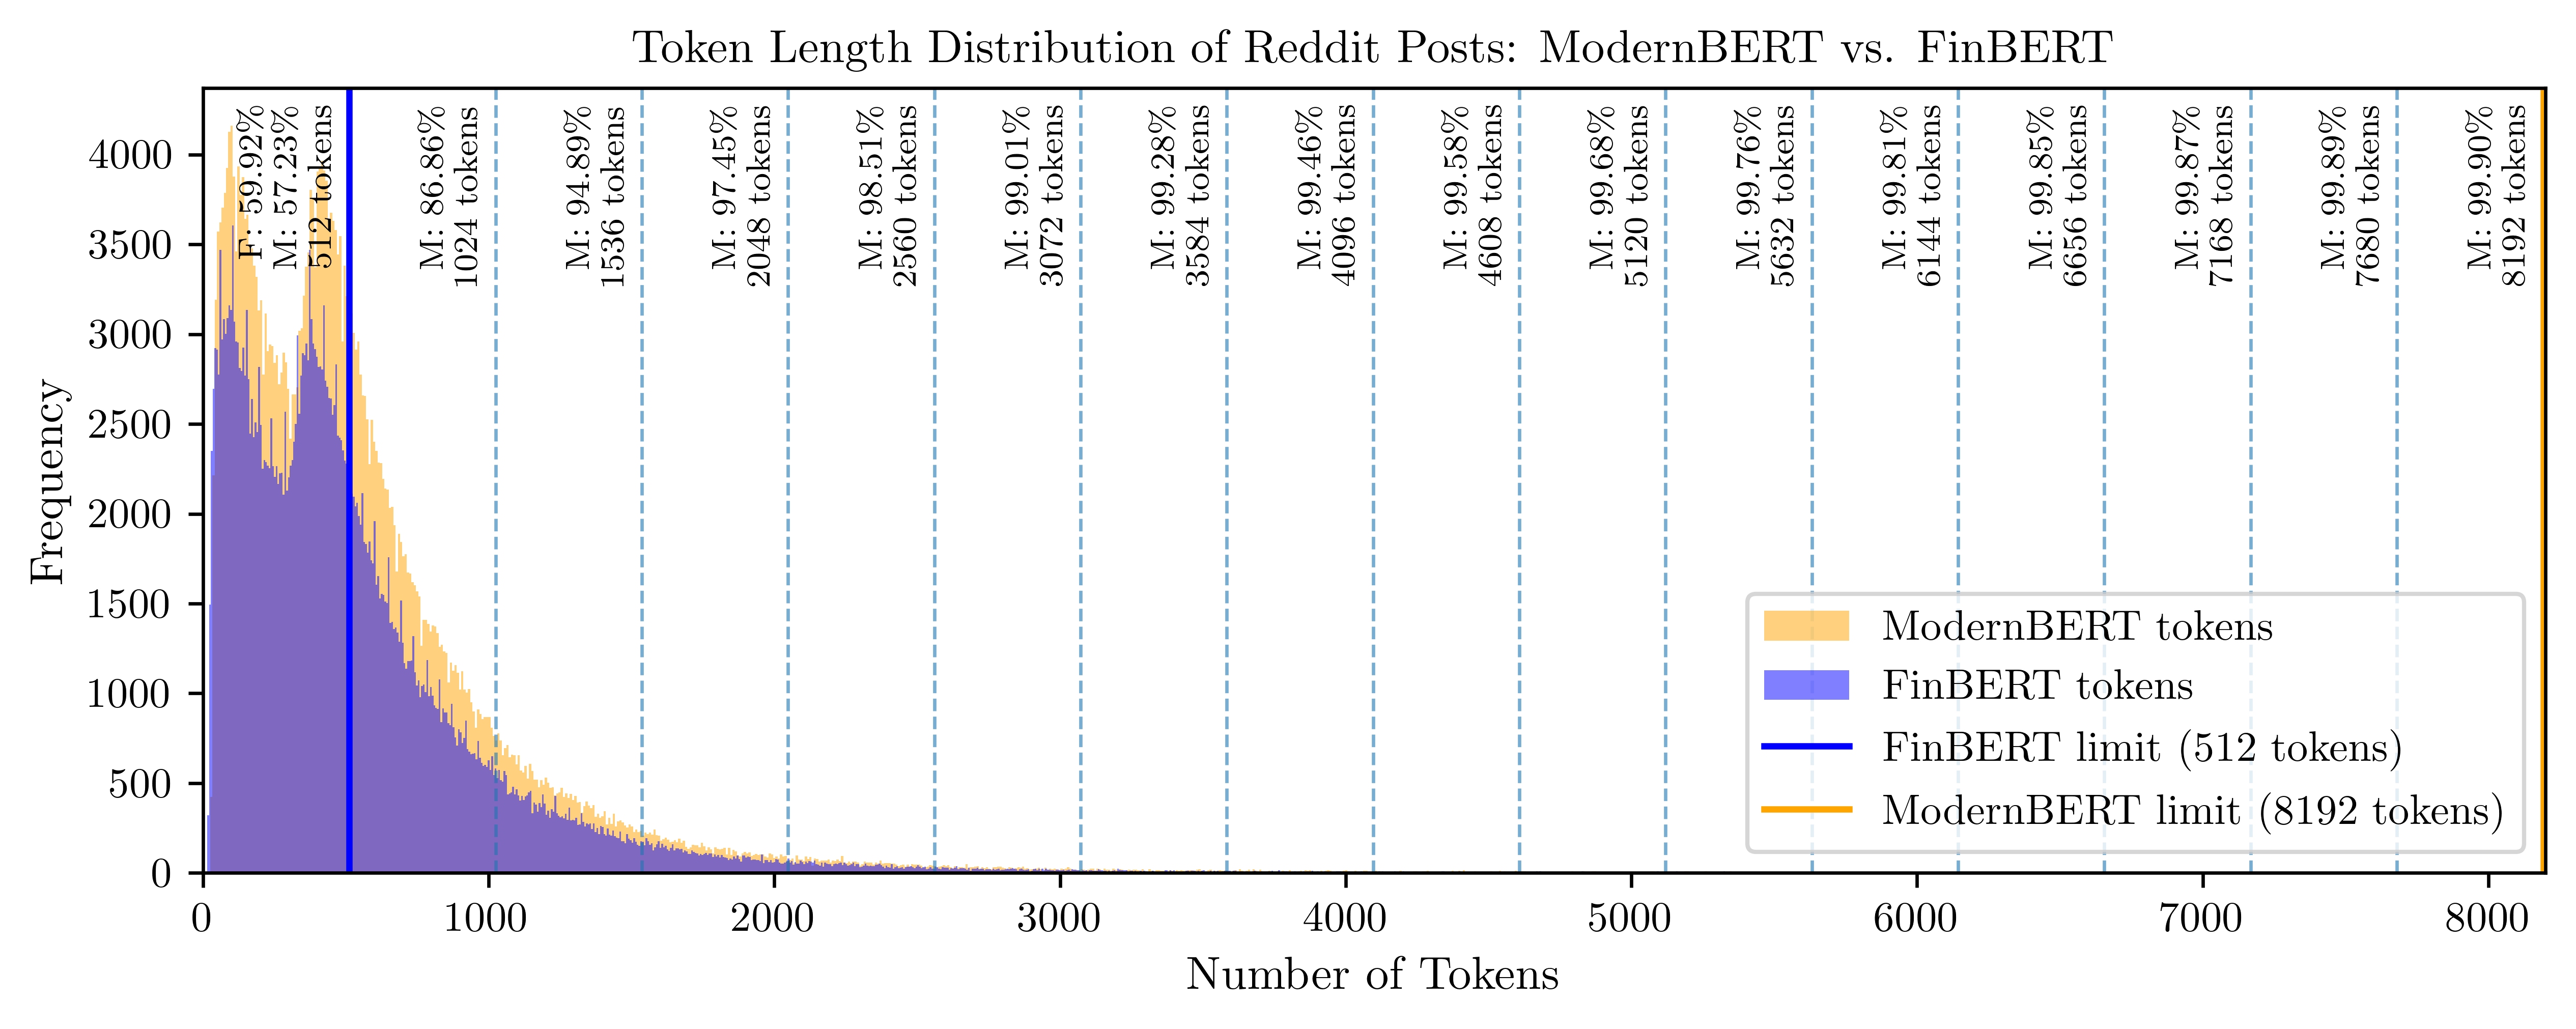
\includegraphics[width=1\textwidth]{figs/reddit_token_distribution.png}
    \caption{Comparative token length distribution of Reddit threads using ModernBERT (M) and FinBERT (F) tokenizers. Vertical dashed lines indicate token length thresholds at regular intervals, while solid lines denote the maximum input limits of each model.}
    \label{fig:token_length_distribution}
\end{figure}

A further challenge was the large number of tokens in many Reddit threads, which frequently exceeded the maximum input length of \texttt{ProsusAI/FinBERT}. Consequently, \texttt{answerdotai/ModernBERT-base}~\cite{modernbert} was selected as a replacement. As shown in Fig.~\ref{fig:token_length_distribution}, FinBERT's $\num{512}$-token limit accommodates only approximately 60\% of threads without truncation, whereas ModernBERT's $\num{8192}$-token limit enables processing of nearly 100\% of threads in full, preventing the loss of contextual information that would otherwise negatively impact classification performance.

The trained model achieved a macro-F1 score of 0.77 on the test set, representing good performance given the complexity of the multi-label, multi-sector classification task and the size of the training dataset. Notably, per-sector performance exhibits considerable variance, with Utilities achieving a macro-F1 score of 0.46 versus 0.84 for Health Care, consistent with the data scarcity issues identified during the labeling process.

The trained model was subsequently applied to the entire Reddit dataset, generating per-post, per-sector sentiment scores for use as features in the portfolio optimization models. Fig.~\ref{fig:sentiment_reddit_diagram} illustrates an example of a Reddit thread and the corresponding input and output of the sentiment classification model, showing how each post is processed to yield a vector of sentiment scores across all sectors.

\begin{figure}[ht]
    \centering
    \includegraphics[width=1\textwidth]{figs/sentiment_reddit_pipeline.png}
    \caption{Overview of the Reddit thread sentiment classification pipeline, showing a sample input thread and the predicted sentiment labels and confidence scores generated by the trained ModernBERT-based model for each sector.}
    \label{fig:sentiment_reddit_diagram}
\end{figure}

Further details regarding the prompts used, model architecture, training procedure, and performance metrics are provided in Appendix~\ref{chap:sentiment_reddit}.

\subsubsection{Feature Construction}

With all sentiment classifications generated for the financial news and social media datasets, each document (GDELT quote or Reddit thread) is now linked to one or more associated sectors, and for each sector, it has a sentiment label (positive, neutral, negative) and a confidence score indicating the certainty of the classification. The next step is to construct the sentiment features that will be used as inputs for the portfolio optimization frameworks. This process involves aggregating the classified sentiment information in a way that aligns with the temporal structure of the market data and the trading calendar.

Associated with each document, there is a timestamp indicating its publication time. This information enables alignment of sentiment data with the corresponding market data for each asset on a daily basis. For example, a document about the Real Estate sector published on a given day can be associated with the relevant ETF (XLRE), contributing to the sentiment features for that asset on that day. Since timestamps were recorded in Coordinated Universal Time (UTC), they were converted to Eastern Time (ET), the time zone of the New York Stock Exchange, the exchange on which the ETFs are traded, to ensure proper alignment with the trading calendar. The strategy assumes daily rebalancing, meaning all portfolio decisions are made once per day using only information available beforehand. Consequently, sentiment data from documents published after the market open (9:30~AM ET) on a given trading day were considered in the following day. This ensures that no look-ahead bias is introduced and that the sentiment features used to determine each day's positions reflect only information that could realistically have been acted upon at the time of trading.

For each asset and each source of sentiment data (GDELT and Reddit), a set of sentiment indicators is designed to capture both current-day sentiment (the \textit{Live} bucket), lagged or rolling sentiment signals (the \textit{Historical} bucket), and missing source data (the \textit{Availability} bucket). Table~\ref{tab:feature_categories_sentiment} summarizes these categories, together with their usage constraints and a brief description of each indicator. 

While the \textit{Live} indicators are straightforward in origin, directly reflecting the sentiment classification for the current trading day, the \textit{Historical} indicators are motivated not only by the potential predictive power of past sentiment, but also by the exclusion of non-trading days from the \textit{Live} data, since news and Reddit posts published on weekends and holidays would otherwise be lost, their sentiment is instead captured through lagged and rolling indicators. The \textit{Availability} indicator addresses a third concern: the presence of missing sentiment data. For the GDELT news data, which is sampled at 15-minute intervals, certain days exhibited partially or completely missing records, so an empirical 80\% availability threshold was therefore applied, whereby if fewer than 80\% of the expected intraday timestamps were present, the day was flagged as missing and the binary \textit{Availability} indicator set accordingly. For the Reddit data, no missing records were identified, however, significant variation in post volume was observed. Reddit's early years (covered by the training set) saw growing platform adoption, resulting in low post volume, and a marked drop was observed between July and October 2023, likely related to the ``Reddit blackout'' and the introduction of restrictive API pricing that shut down most third-party applications~\cite{redditblackout2023}, though no missing flag was applied as the data was sparse but present.

Additionally, since sentiment classification probabilities are continuous values between 0 and 1, a confidence thresholding mechanism is applied. The threshold is treated as a tuned hyperparameter, taking values of $0.00$, $0.50$, $0.75$, or $0.90$: documents with a classification probability below the threshold are discarded from the computation of sentiment indicators. For example, with a threshold of $0.75$, only documents classified with at least 75\% confidence for a given sentiment class contribute to the indicators. This mechanism controls the trade-off between data coverage (lower threshold) and signal reliability (higher threshold), and can have a significant impact on the quality of the resulting sentiment features.

It is also worth noting, as with the Technical Features, that selecting an indicator (except for the \textit{Availability} one) implies adding 11 features to the model input (one per ETF in the investable universe).

\begin{table}[ht]
\centering
\caption{Summary of the sentiment feature space derived from GDELT quotes or Reddit threads, including live sentiment, historical sentiment, and availability indicators.}
\label{tab:feature_categories_sentiment}
\renewcommand{\arraystretch}{1.2}
\begin{tabular}{|c|c|p{8.5cm}|}
\hline
\textbf{Category} & \textbf{Usage / Features} & \textbf{Description} \\
\hline

Live & Exactly one & Current-day sentiment indicators \\
\cline{2-3}
 & \texttt{balance} & Net sentiment score: sum of positive confidence scores minus sum of negative confidence scores for the day \\
 & \texttt{balance\_ratio} & Ratio of the balance to the total number of positive and negative documents for the day \\
 & \texttt{countPos} \& \texttt{countNeg} & Number of documents classified as positive and negative for the day \\
 & \texttt{ratioPos} \& \texttt{ratioNeg} & Fraction of documents classified as positive and negative out of all documents for the day \\
\hline

Historical & Up to one & Lagged or rolling sentiment indicators \\
\cline{2-3}
 & \texttt{BR\_Rolling3} & 3-day rolling mean of the daily balance ratio \\
 & \texttt{BR\_Rolling5} & 5-day rolling mean of the daily balance ratio \\
 & \texttt{BR\_Rolling22} & 22-day rolling mean of the daily balance ratio \\
 & \texttt{BR\_Lag1} \& \texttt{BR\_Lag5} & Balance ratio lagged by 1 and 5 trading days \\
 & \texttt{BR\_Var1} \& \texttt{BR\_Var5} & Day-over-day and 5-day change in the balance ratio \\
\hline

Availability & Mandatory & Indicator of whether source data was available \\
\cline{2-3}
 & \texttt{is\_missing} & Binary indicator for missing source data \\
\hline

\end{tabular}
\end{table}

The neutral sentiment class was excluded from the feature construction process, as reflected by the absence of a corresponding indicator in Table~\ref{tab:feature_categories_sentiment}. This decision was motivated by the fact that neutral sentiment constituted most classified documents, approximately 61\% for GDELT quotes and 96\% for Reddit threads, largely because it functioned as a default label when no meaningful connection to a sector was identified. Including this class would have introduced additional dimensionality and complexity without contributing useful information. More importantly, neutral sentiment lacks directional insight into market attitudes, making it less relevant for predictive modeling. By removing it, the feature set is streamlined to focus on positive and negative sentiment indicators, which are more informative and better suited to influencing the portfolio optimization process.